\documentclass[a4paper,12pt]{report} %размер бумаги устанавливаем А4, шрифт 12пунктов

\usepackage[T2A]{fontenc}
\usepackage[utf8]{inputenc}%включаем свою кодировку: koi8-r или utf8 в UNIX,
\usepackage[english,russian]{babel}%используем русский и английский языки с переносами
\usepackage{amssymb,amsfonts,amsmath,mathtext,cite,enumerate,float} %подключаем нужные пакеты расширений
\usepackage{graphicx} %хотим вставлять в диплом рисунки?
\usepackage{indentfirst}
\usepackage{geometry} % Меняем поля страницы

\bibliographystyle{utf8gost705u}
\bibliographystyle{unstr}

\makeatletter
\makeatother

\geometry{left=2cm}% левое поле
\geometry{right=1.5cm}% правое поле
\geometry{top=1cm}% верхнее поле
\geometry{bottom=2cm}% нижнее поле


\title{Использование GPIO на Cubieboard 1|2.}
\date{}
\author{Степанов~А.~О.}

\begin{document}
	
	\maketitle
	
	\tableofcontents % это оглавление, которое генерируется автоматически
	
	\newpage
	
	\section{Что такое GPIO.}
		\begin{figure}[h]
			\center{
				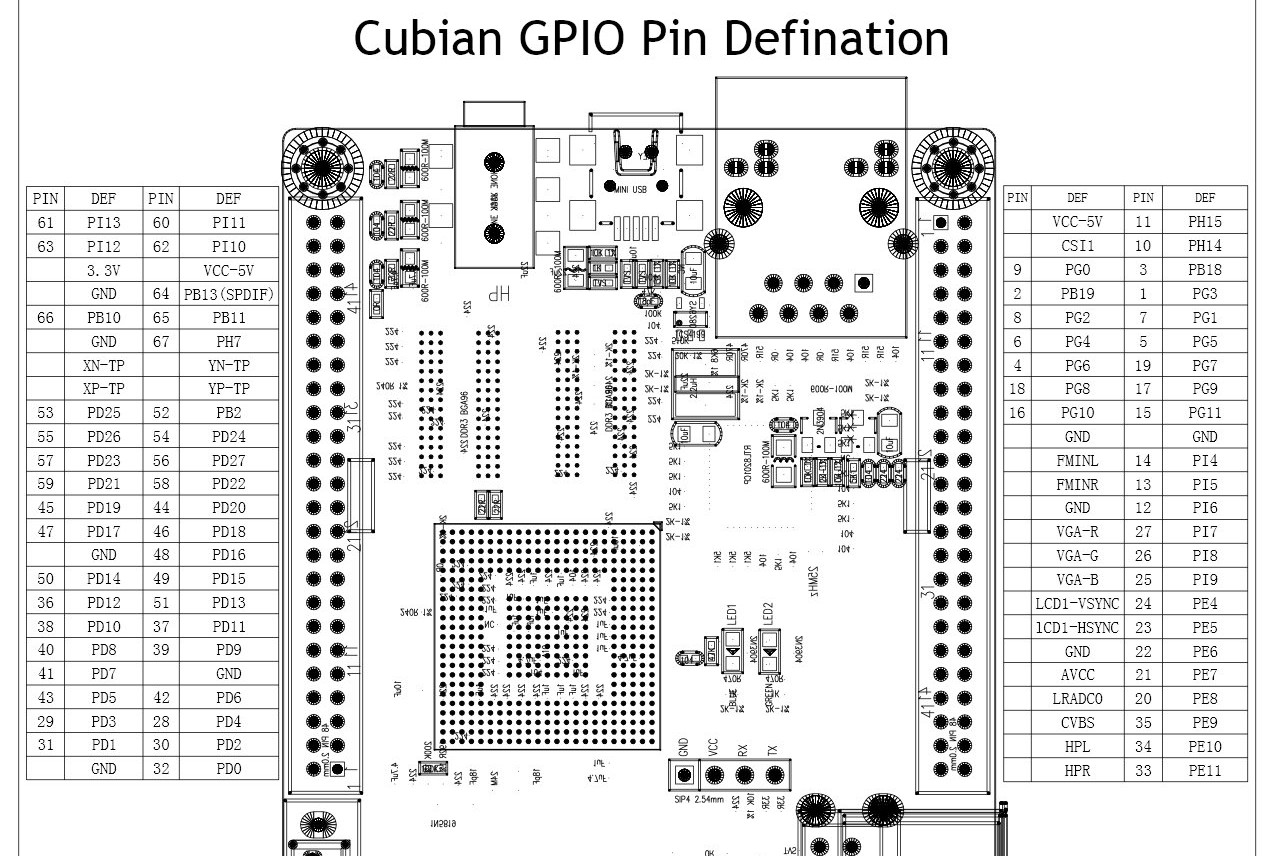
\includegraphics[scale=0.8]{gpio_defination_large.jpg}
			}
			\caption{Номера и названия портов GPIO на плате}
			\label{ris:gpio}
		\end{figure}
		GPIO(General-purpose input/output) - это ряд специальных контактов общего
		назначения, пользователь может определить для каждого из них является ли он
		входом, либо выходом.\cite{wiki}
		По умолчанию назначения не определены.
		Возможности GPIO:
		\begin{enumerate}
		  \item{может быть сконфигурировани для ввода или вывода}
		  \item{GPIO контакты могут быть отключены}
		  \item{на выходе может быть или 1 или 0}
		  \item{можно изменять выходные значения}
		  \item{часто можно использовать систему прерываний для GPIO} 
		\end{enumerate}
		
	\section{Особенности GPIO в Cubieboard 1|2.}
	
	Рассмотрите Рис. ~\ref{ris:gpio}. Название линии GPIO имеет вид P\{имя
	порта\}\{номер пота\}.
	Графа PIN - это номер, по которому к нему можно обратиться из системы. Как видно из рисунка, не
	все линии можно испольовать для чего угодно, некоторые из них уже задействованы
	в конфиигурации системы.\cite{hub}
	Линии, помеченные как VCC-5V и 3.3V - это выводы для питания. Линии GND - земля.
	Здесь же распаяны интефейсы VGA, SPI и другие.
	Стоит обратить внимние, что растояние между штырками в Cubieboard гораздо меньше
	чем Paspberry PI или Arduino, это надо учитывать при выборе контактов для
	подключения.
	\section{Использование GPIO в ОС Linux.}
		\subsection{Общие момоенты.}
			Прочитать подробно о GPIO в Linux можно в документе [LGIO00]
			GPIO в Linux после загрузки принадлежит системе, и для его использования каждую
			линию необходимо экспортировать. Для этого в каталоге \emph{/sys/class/gpio}
			в специальный файл \emph{export} необходимо послать номер нужной линии.
			Например для открытия линии 17, которая отвечает порту G9 (PG9) Рис.~\ref{ris:gpio}:
			Код на bash:
			\begin{verbatim}
			# echo 17 > /sys/class/gpio/export
			\end{verbatim}
			Код на C:
			\begin{verbatim}
			write(fd, "17", 1);
			\end{verbatim}
			Если команда выполнилась успешно, то в дирректории \emph{/sys/class/gpio}
			появится дирректория \emph{gpio17\_pg9}. В ней есть файлы:
			\begin{enumerate}
			  \item{direction - определяет направление линии: является ли она входом или
			  выходом, чтобы настроить линиюнужно записать в фал слово 'in' или 'out'
			  соответственно. Например:
				  \begin{verbatim} 
				  	# echo out > /sys/class/gpio/gpio17/direction
				  \end{verbatim}}
			  \item{value - позволяет прочитать или считать значение с линии, в зависимости
			  от того, какой тип в direction записан, in или out соответственно Например
			  запись: 
				  \begin{verbatim} 
				  	# echo 1 > /sys/class/gpio/gpio17/value
				  \end{verbatim} 
				  Или чтение: 
				\begin{verbatim} 
					# cat /sys/class/gpio/gpio17/value
				\end{verbatim} 
				Внимание! Это символы а не числа!}
			  \item{edge - управляет котроллером прерываний. 
			  	\begin{enumerate}
				  \item{none - выключет отслеживание изменения состояния входящей линии;}
				  \item{rising - отслеживает переход из неактивного состояния в активное;}
				  \item{falling - отслеживает переход из активного состояния в неактивное;}
				  \item{both - реагирует на любые изменения состояния.}
				\end{enumerate}}
			  \item{active\_low - уровень активного сигнала, то есть напряжение логических
			  нуля и единицы. По умолчанию в Cubieboard 1 - 3.3V, а 0 - 0V. Записанная сюда
			  единица инвертирует активный сигнал}
			\end{enumerate}
			\subsection{Запись.}
				\begin{figure}[h]
					\center{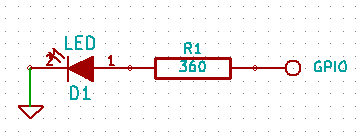
\includegraphics[scale=0.8]{led.png}}
					\caption{Подключение светодиода к GPIO}
					\label{ris:led}
				\end{figure}
				Возьмем простой пример, нам необходимо зажигать или выключать светодиод,
				подключенный по схеме Рис.~\ref{ris:led}
				В качестве GPIO можно взять любой, пусть это будет 17. Включаем линию:
				\begin{verbatim}
				# echo 17 > /sys/class/gpio/export
				\end{verbatim}
				Задаем ей направление на выход:
				\begin{verbatim}
				# echo out > /sys/class/gpio/gpio17_pg9/direction
				\end{verbatim}
				Включаем 17-й, т. е. подаем на него напряжение:
				\begin{verbatim}
				# echo 1 > /sys/class/gpio/gpio17_pg9/value
				\end{verbatim} 
				Выключаем 17-й:
				\begin{verbatim}
				# echo 0 > /sys/class/gpio/gpio17_pg9/value
				\end{verbatim} 
		\subsection{Чтение.}
			\begin{figure}[h]
				\center{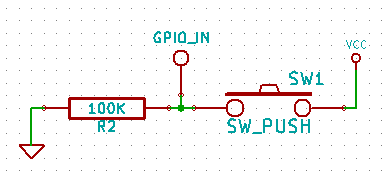
\includegraphics[scale=0.8]{but.png}}
				\caption{Подключение светодиода к GPIO}
				\label{ris:but}
			\end{figure}
			Теперь чтение по схеме на Рис.~\ref{ris:but}:
			Аналогично в качестве \emph{GPIO\_IN} можно взять любой, пусть это опять будет
			17.
			Включаем линию:
			\begin{verbatim}
			# echo 17 > /sys/class/gpio/export
			\end{verbatim}
			Задаем ей направление на вход:
			\begin{verbatim}
			# echo in > /sys/class/gpio/gpio17_pg9/direction
			\end{verbatim}
			Считываем значение:
			\begin{verbatim}
			# cat /sys/class/gpio/gpio17_pg9/value
			\end{verbatim} 
			Полученное значение зависит от \emph{active\_low}, если его не меняли, то мы
			получим символ(!) 1, если кнопка нпжата и 0 в противном случае. Соединение с землей
			нужно для предотвращения появления 1 на висящем в воздуже выводе.
		\subsection{Использование прерываний GPIO.} 
			Для использования прерываний, необходимо активировать линию и записать способ
			слежения в \emph{edge}. Повторюсь:
			\begin{enumerate}
			  \item{none - выключет отслеживание изменения состояния входящей линии;}
			  \item{rising - отслеживает переход из неактивного состояния в активное;}
			  \item{falling - отслеживает переход из активного состояния в неактивное;}
			  \item{both - реагирует на любые изменения состояния.}
			\end{enumerate}
			По инструкции, достаточно выбрать оди из способов кроме \emph{none} и значение
			можно будет считывать с помощью \emph{poll()} или \emph{select()}. В случае,
			если значение изменилось, вызов \emph{read()} должен быть заблокирован, но этого
			не произойдет. Так сделанно для работы команды \emph{cat value}. \cite{habr}
			Из всего этого алгоритм звучит примерно так: 
			\begin{enumerate}
			  \item открыть файл \emph{value};
			  \item читать из него начальное значение(теперь файл будет блокироваться).
			\end{enumerate}
			Есть еще одна тонкость: значения читаются только по смещению 0, в то время как
			вызов функции \emph{read()} меняет позицию чтения. Поэтому позицию чтения
			необходимо сбромить с помощью \emph{lseek()}. В итоге примерно так выглядит
			чтение GPIO с использованием событий \emph{edge}:
			\begin{verbatim}
			// выбор способа отслеживания
			int gpio_edge_set(int n, const char *edge_str)
			{
			    char filename[PATH_MAX];
			    FILE *file;
			    snprintf(filename, sizeof(filename), "/sys/class/gpio/gpio%d/edge", n);
			    file = fopen(filename, "w");
			    if (file == NULL) return -1;
			    fprintf(file, "%s\n", edge_str);
			    fclose(file);
			
			    return 0;
			}
			
			// pool()
			int gpio_poll(int n)
			{
			    char filename[PATH_MAX];
			    int fd;
			    char c;
			    int err;
			
			    snprintf(filename, sizeof(filename), "/sys/class/gpio/gpio%d/value", n);
			    fd = open(filename, O_RDONLY);
			    if (fd < 0) return -1;
			
			    read(fd, &c, sizeof(c));
			
			    return fd;
			}
			
			// получение значения с линии
			int gpio_get(int fd, int timeout)
			{
			    struct pollfd pollfd[1];
			    char c;
			    int err;
			
			    pollfd[0].fd = fd;
			    pollfd[0].events = POLLPRI | POLLERR;
			    pollfd[0].revents = 0;
			
			    err =  poll(pollfd, 1, timeout);
			    if(err != 1) return -1;
			
			    lseek(fd, 0, SEEK_SET);
			    err = read(fd, &c, sizeof(c));
			    if(err != 1) return -1;
			
			    return c - '0';
			}
			\end{verbatim} 
		
		\bibliography{biblio}

\end{document} 
